\documentclass{article}
\usepackage[utf8]{inputenc}
\usepackage{graphicx}
\usepackage{parskip}

\graphicspath{ {./images/} }

\frenchspacing

\title{Santa's Little Cookbook}

\begin{document}

\maketitle

\vspace{3cm}
\begin{center}

\includegraphics[width=0.5\textwidth]{logo}
\end{center}

\newpage
\section{Meatloaf (fasírt)}

A bit different from the traditional Hungarian meatloaf recipe, this version is more suited to be cut and eaten cold (as a sandwich, for instance, or with some salad as a side). It's fairly quick and simple to make. 

\subsection{Ingredients}
\begin{itemize}
    \item 1kg minced meat (pork or beef)
    \item 5 eggs
    \item a larger onion
    \item a couple of cloves of garlic
    \item breadcrumbs
    \item marjoram, salt, pepper
    \item lard or olive oil
\end{itemize}

\subsection{Directions}
Let's start with the difficult part: grate the onion. Yeah, that's right, grate that sucker, ho ho ho! It seriously tastes better that way, and helps with the smooth consistency we're going for.

\begin{figure}[!htbp]
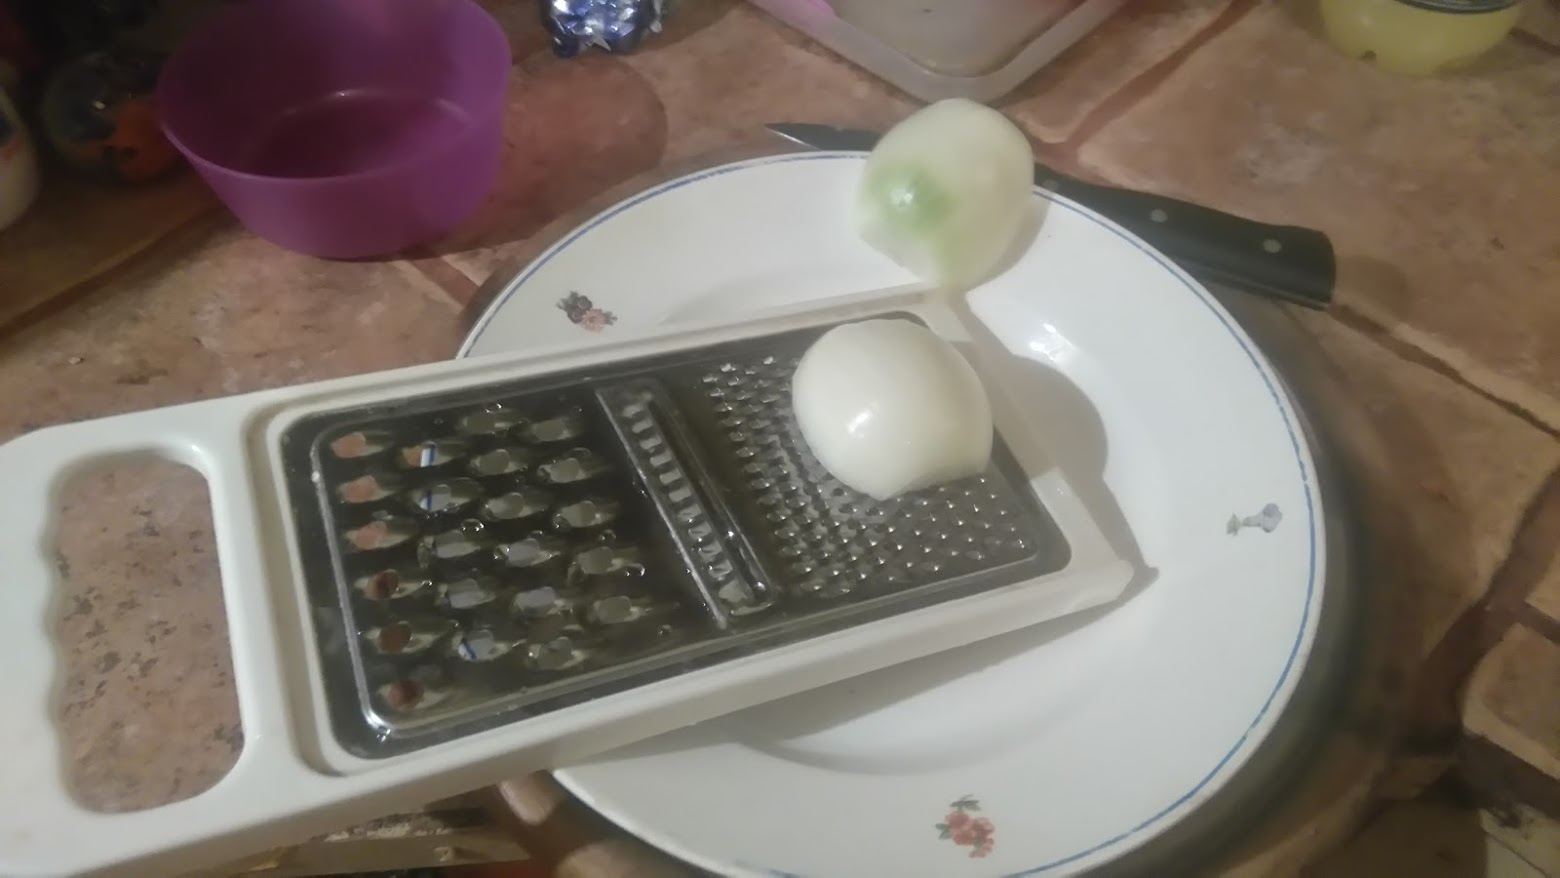
\includegraphics[width=\textwidth]{meatloaf_01}
\caption{Grating onions is a bit of a hassle}
\end{figure}

Now get your eggs ready: crack them all into a dish and beat them (beat 'em real good ho ho ho). Make sure to add a bit of salt.

\begin{figure}[!htbp]
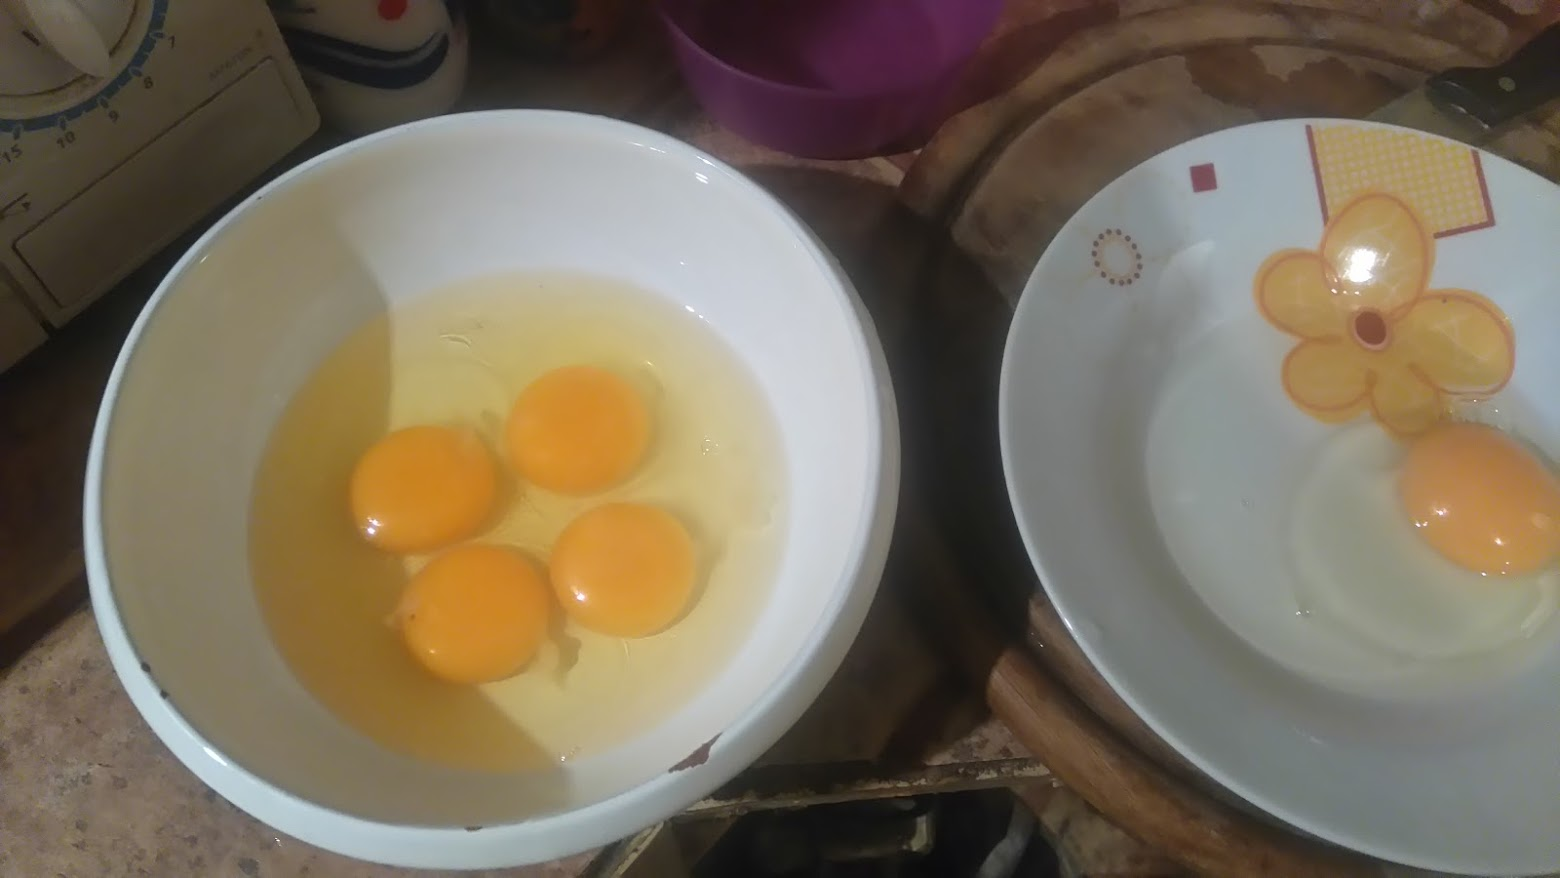
\includegraphics[width=\textwidth]{meatloaf_03}
\caption{Eggs, yet unbeaten}
\end{figure}

This may be a good time to crush your garlic. You may try mincing if you don't have a garlic press, but crushed garlic is just better (ho ho ho ho).

Put the minced meat in a bowl, add a generous amount of salt and pepper. Also add marjoram: it's a wonderful spice.

Now would be a good time to get the oven going. A medium heat of around 180 degrees is best.

\begin{figure}[!htbp]
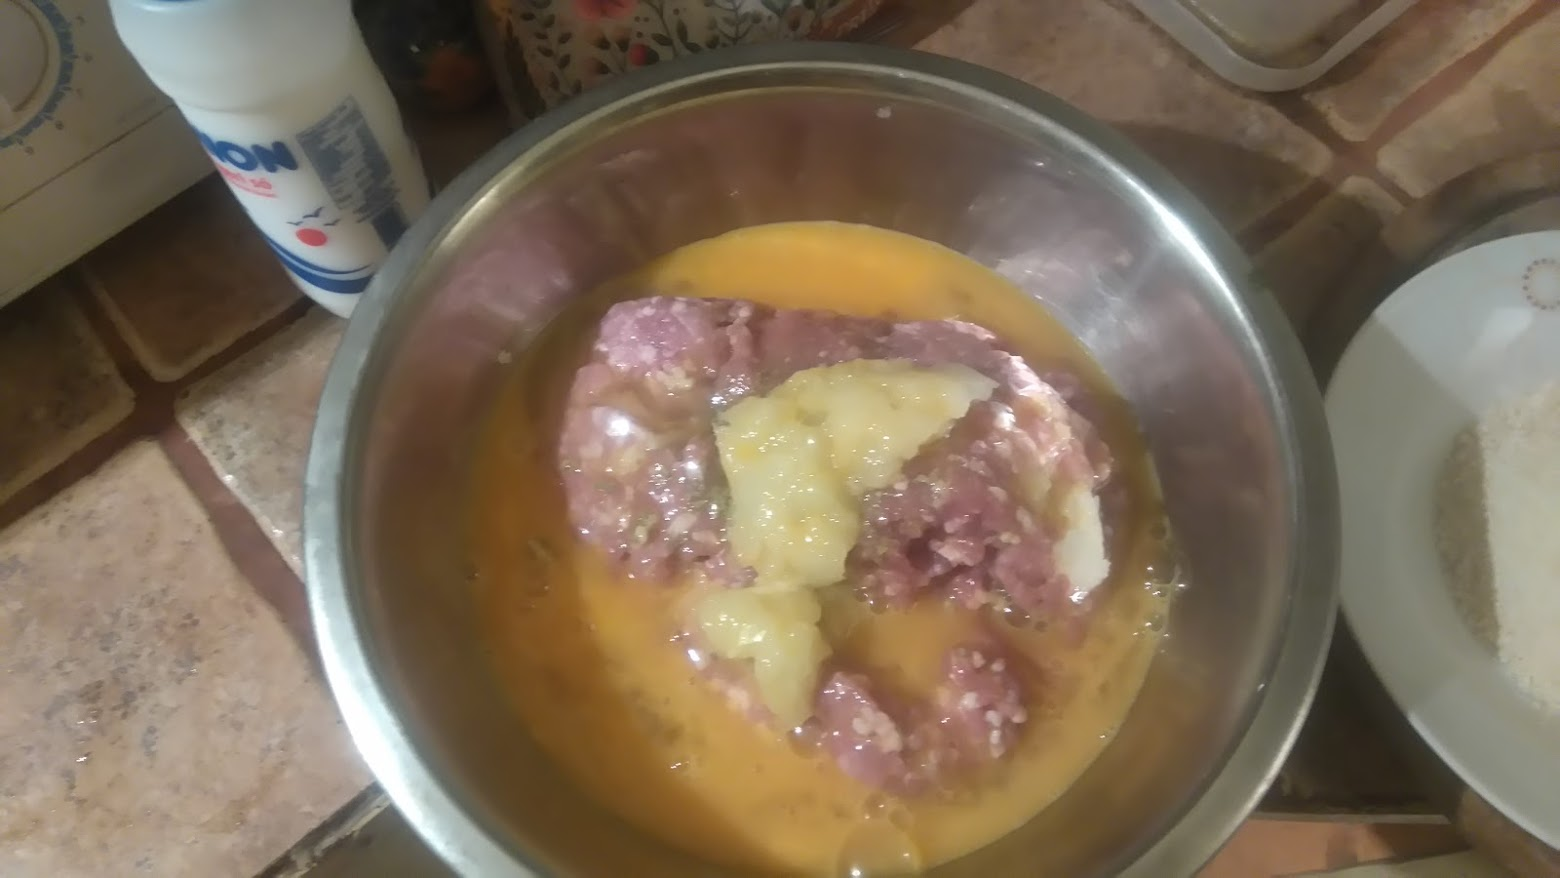
\includegraphics[width=\textwidth]{meatloaf_09}
\caption{Just dump all the ingredients in a bowl}
\end{figure}

And now comes the best part: we can start mixing the ingredients. Just dump the eggs, the grated onions and the crushed garlic on top of the meat, and start mixing it, using your impeccably clean hand.

As you're massaging the mixture, start adding the breadcrumbs. It's best to make the breadcrumbs by grating old bread, but store-bought breadcrumbs are fine as well. Keep adding breadcrumbs and keep mixing until the mixture reaches the desired consistency: smooth, homogeneous.

\begin{figure}[!htbp]
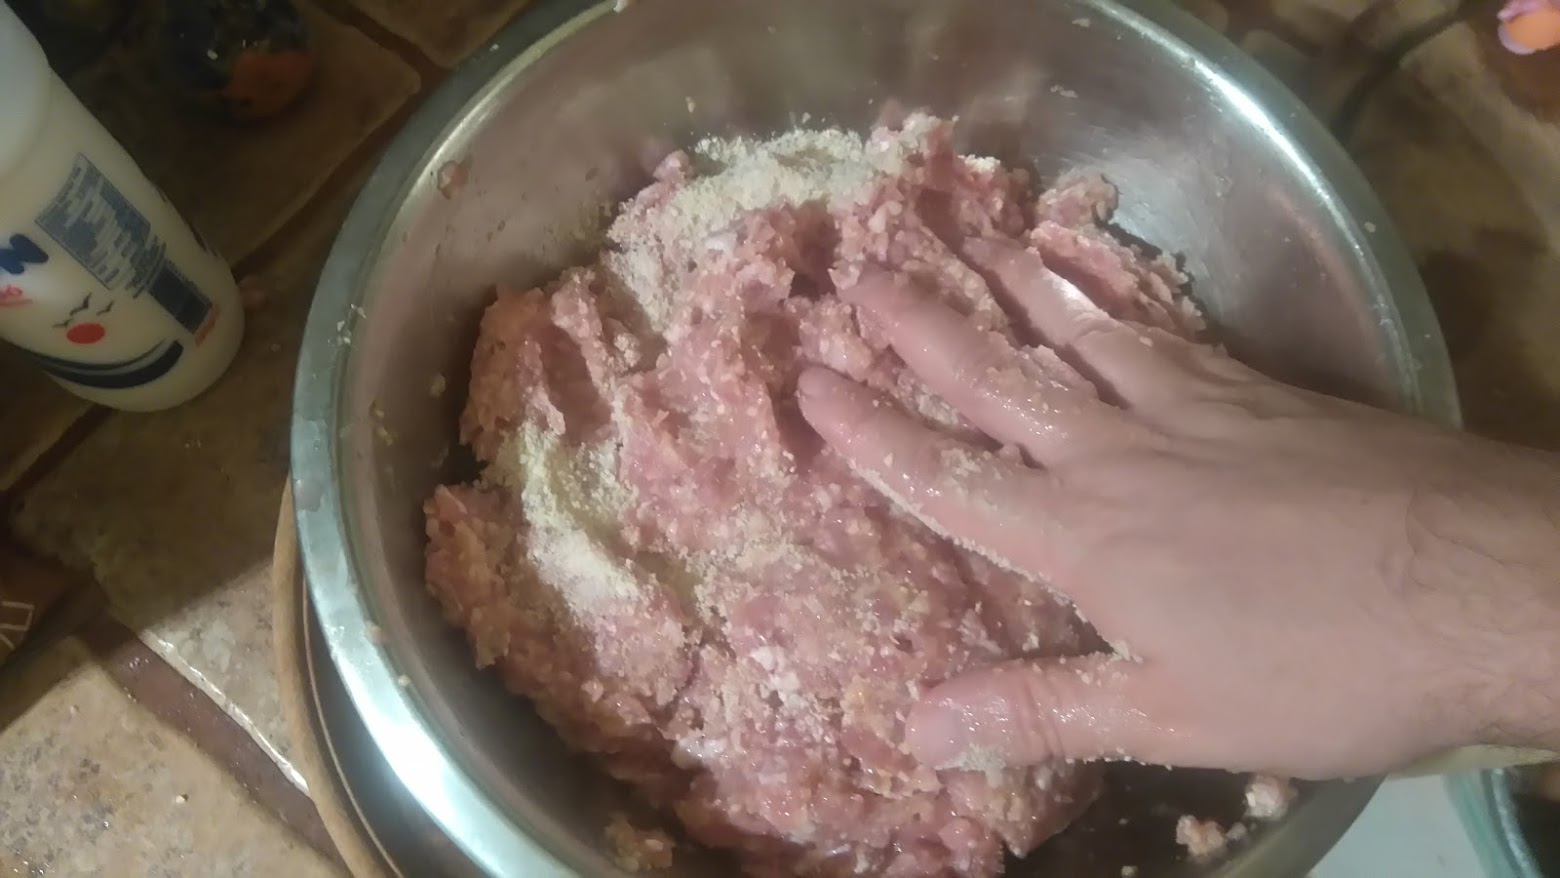
\includegraphics[width=\textwidth]{meatloaf_11}
\caption{Massaging the mixture is kinda fun.}
\end{figure}

Don't forget the salt: traditionally the raw mixture is tasted to ensure it's salty enough, but this Santa has always been too squeamish to do that. Anyhow.

Form the mixture into a longish, fat little shape, and put it on the oven pan. Massage it into a square-ish shape. Smear a bit of lard or olive oil over it, then put a bit of water (around 1.5 dl) into the pan. 

\begin{figure}[!htbp]
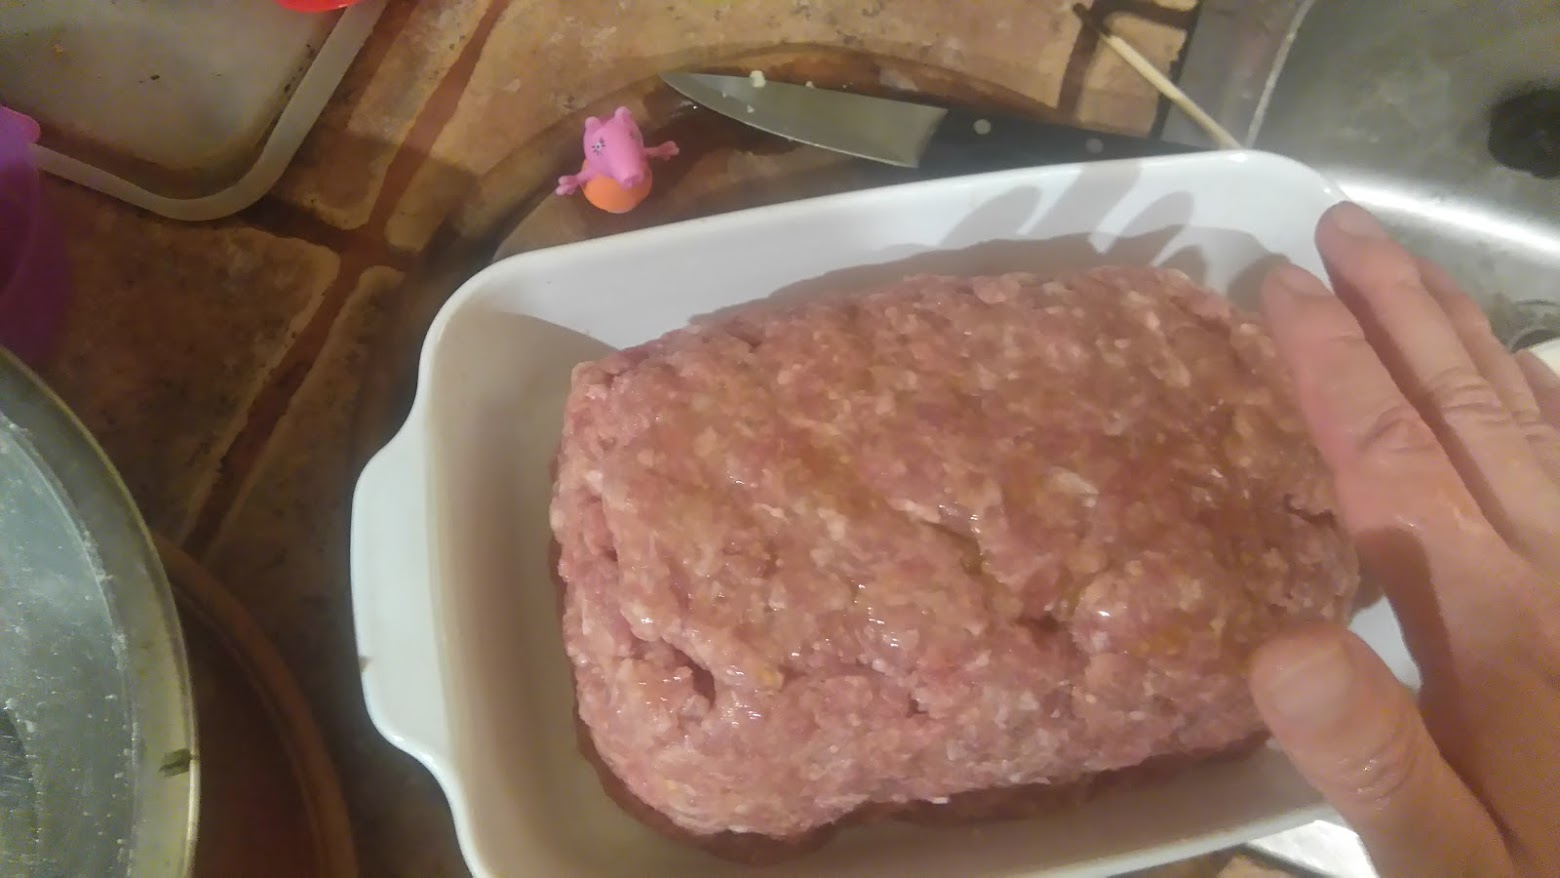
\includegraphics[width=\textwidth]{meatloaf_13}
\caption{The meatloaf in the oven pan.}
\end{figure}

Put the pan into the oven and let it bake until it turns a nice brown colour. If unsure, test it with a fork in the usual way: the meatloaf is ready if no liquid runs out when stabbed.

\begin{figure}[!htbp]
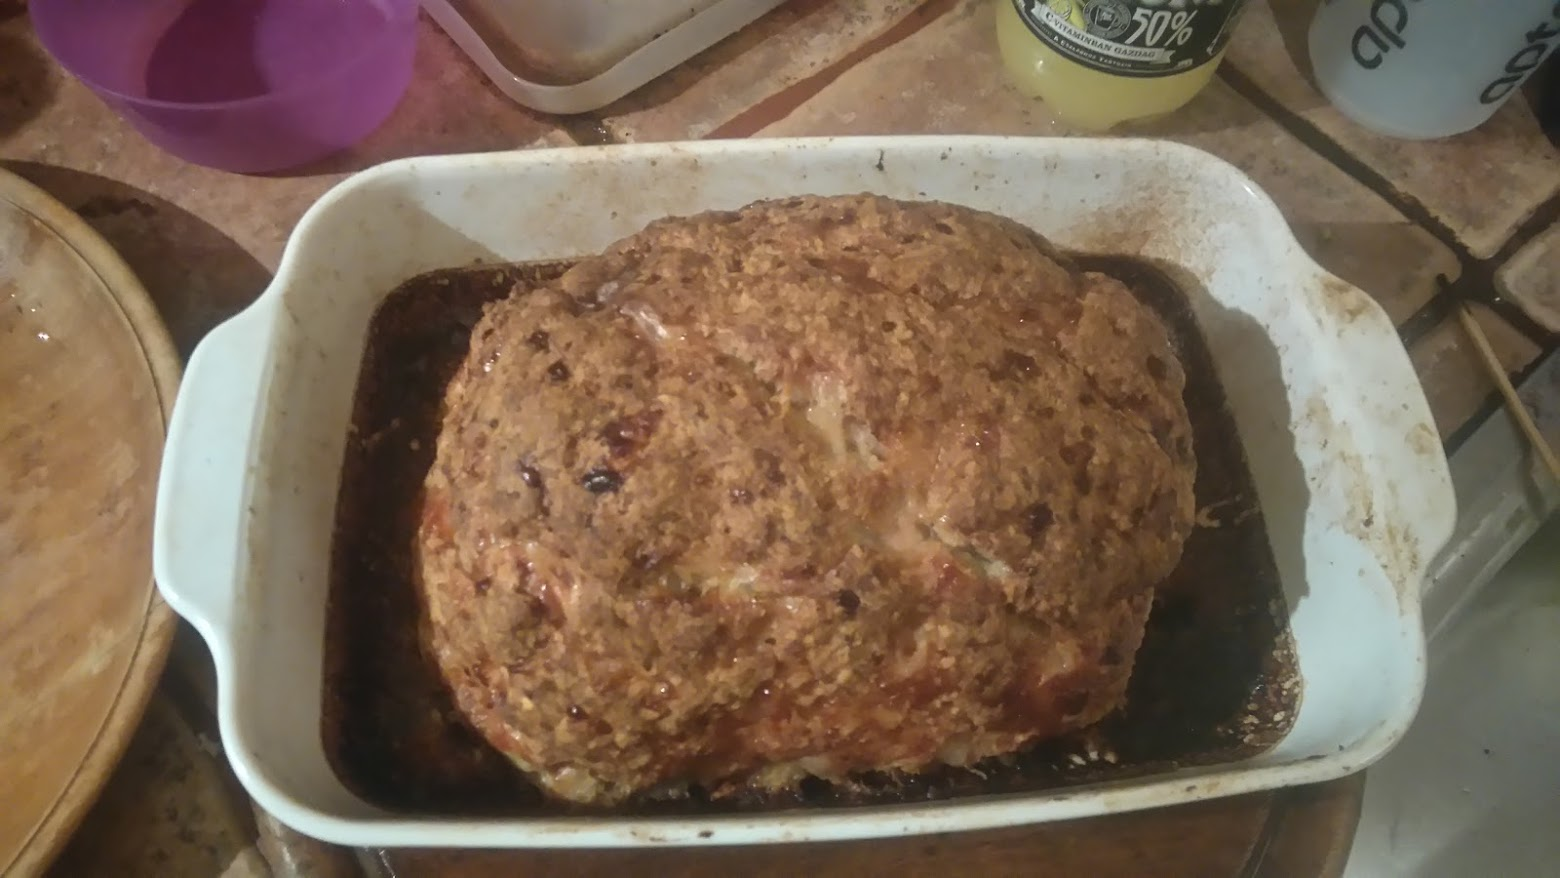
\includegraphics[width=\textwidth]{meatloaf_17}
\caption{And it's done!}
\end{figure}

Ideally let it cool a bit before cutting slices.

\newpage
\section{Rice cake (rizskoch, rizsfelfújt)}

This is the only dessert I can make reliably. A real comfort food.

\subsection{Ingredients}

\begin{figure}[!htbp]
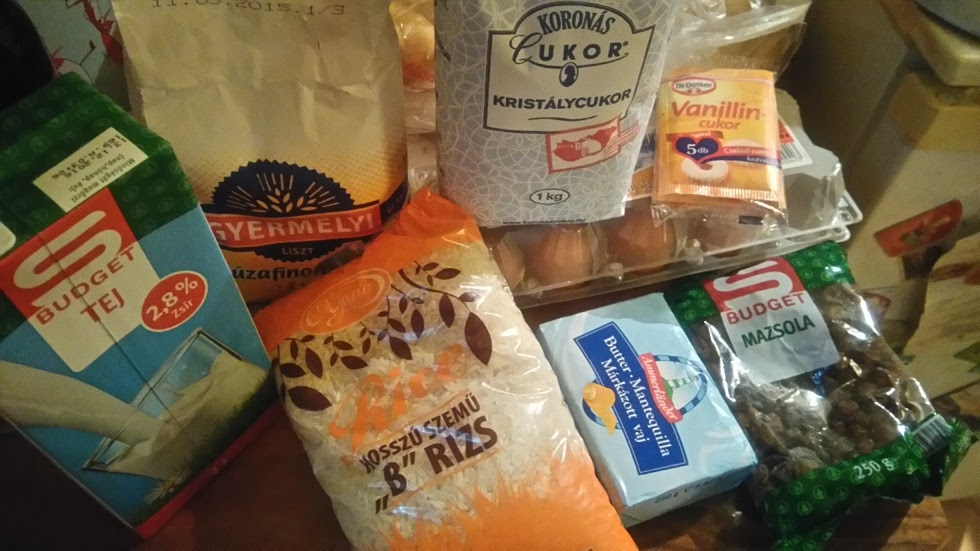
\includegraphics[width=\textwidth]{rizskoch_01}
\caption{Collected ingredients}
\end{figure}

\begin{itemize}
    \item 30dkg rice
    \item 2dl water
    \item 1l milk
    \item 6 eggs
    \item 5dkg butter
    \item 20dkg sugar
    \item 2 packets of vanillin
    \item ~10dkg raisins
    \item a bit of flour
\end{itemize}

\subsection{Directions}

Wash the rice carefully in cold water, then let it dry.

\begin{figure}[!htbp]
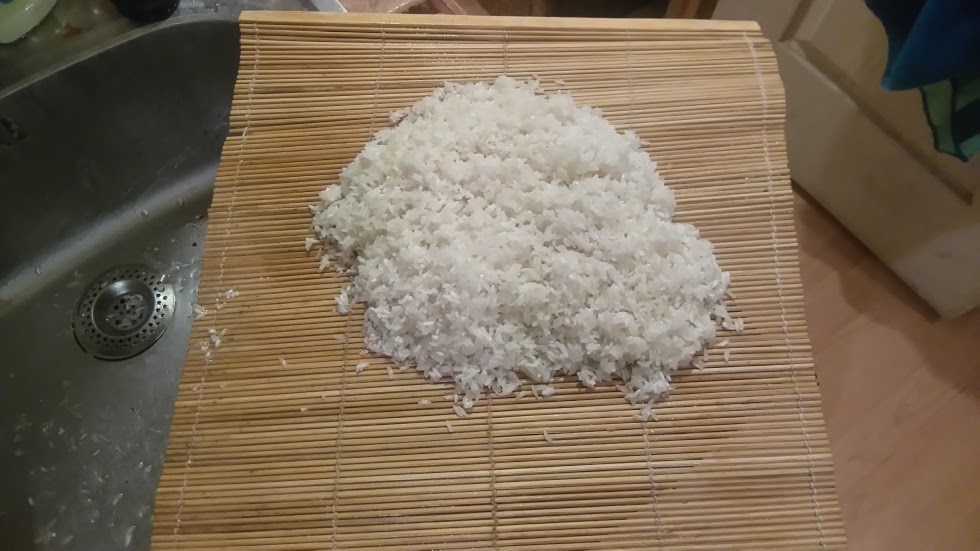
\includegraphics[width=\textwidth]{rizskoch_02}
\caption{Washed rice drying}
\end{figure}

Also wash the raisins and set it aside.

Boil 2dl of water in a pan, put the rice in. Keep stirring until almost no water is left. Pour in 8dl of the milk, add the butter (broken up into pieces), add 2 tablespoons of sugar and a pinch of salt. You may want to add a bit of lemon rind or lemon zest.

\begin{figure}[!htbp]
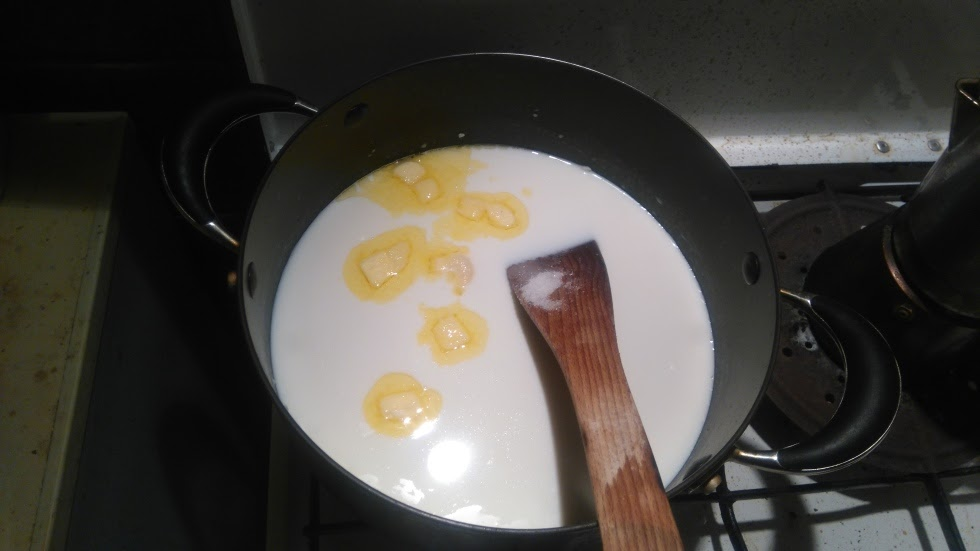
\includegraphics[width=\textwidth]{rizskoch_04}
\caption{Cook the rice in milk, with butt and sugar added}
\end{figure}

Keep stirring, and cook until the rice is fully soft. Get the pan off the heat and mix the raisins in\footnote{This Santa has met a couple of people who dislike raisins. Well, if you're one of those people, you may substitute some other dried fruit, or leave it off entirely}. Don't be alarmed if it looks too thin, watery, that's expected. Cover the pan and set it aside, leaving it to cool for at least an hour.

While our mixture is cooling off, crack the eggs, separating the yolk and the whites. Beat the whites until very stiff\footnote{Adding a tiny bit of lemon juice helps}. Take the yolks and mix them with 20dkg sugar. This may be a good time to heat the oven to medium heat (180-200 degrees).

\begin{figure}[!htbp]
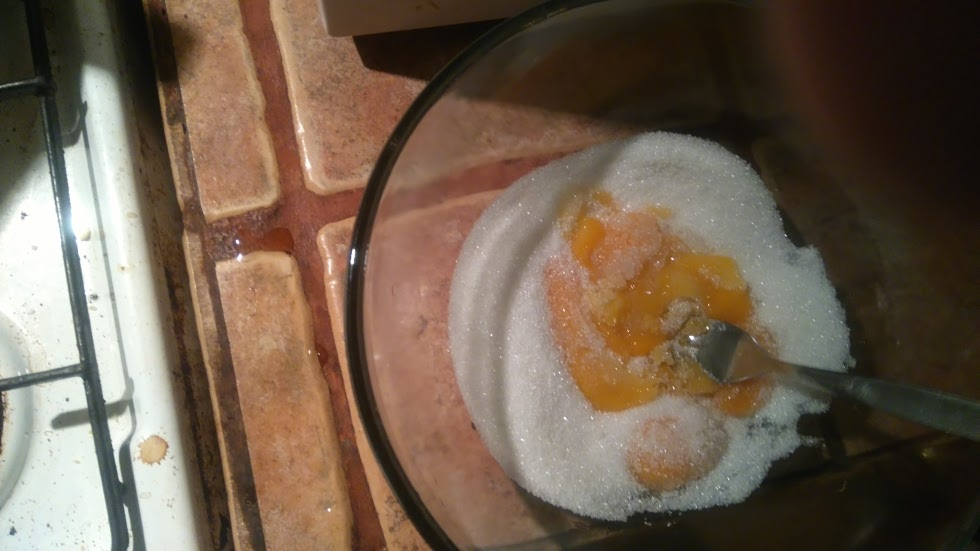
\includegraphics[width=\textwidth]{rizskoch_08}
\caption{Egg yolk and sugar}
\end{figure}

The rice-milk mixture must have turned pretty solid while cooling off. Pour the rest of the milk on it and stir to make it easier to handle. Mix in the sugary egg yolk. Then mix in the beaten egg white very carefully. Very-very carefully.

\begin{figure}[!htbp]
\centering
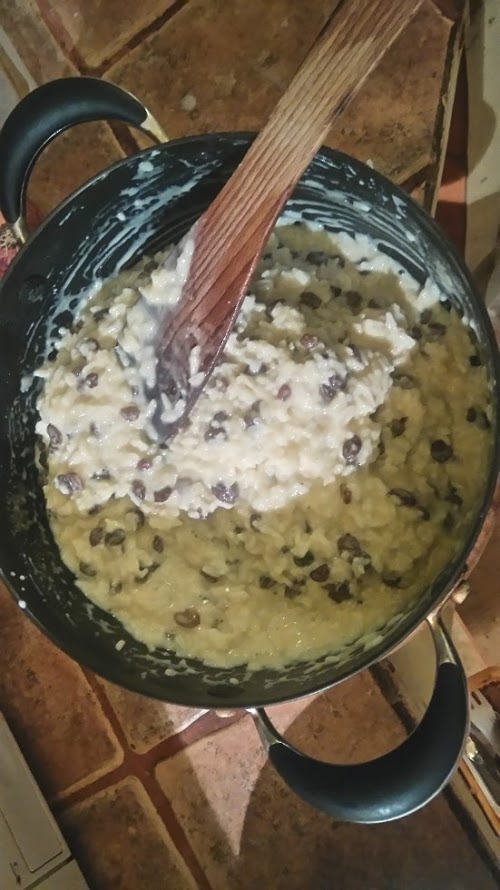
\includegraphics[height=\textwidth]{rizskoch_13}
\caption{The mixture has solidified after cooling off}
\end{figure}

Lightly butter and flour your favourite oven pan, then carefully pour the mixture in it. 

\begin{figure}[!htbp]
\centering
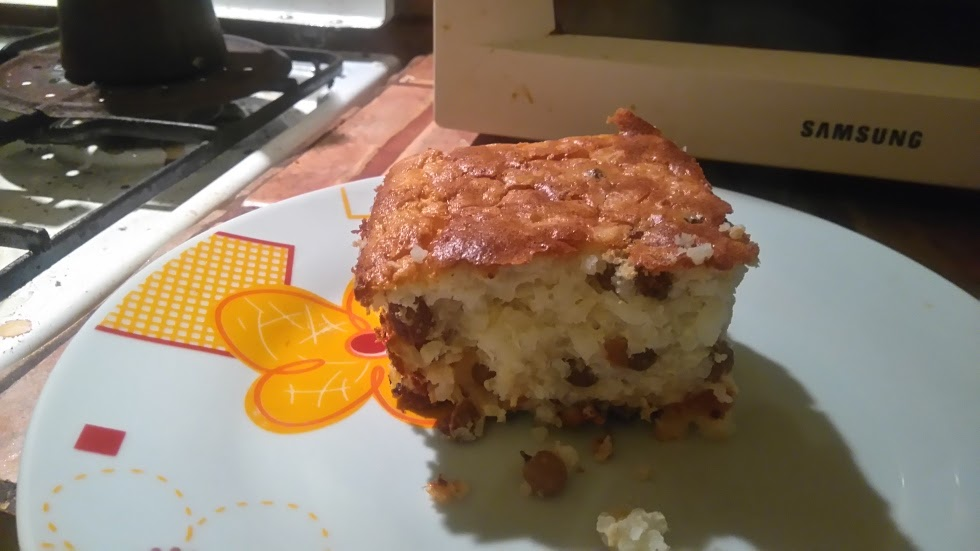
\includegraphics[width=\textwidth]{rizskoch_16}
\caption{/r/boneappletea}
\end{figure}


Put the pan in the oven and cook until the top turns golden brown. Optionally sprinkle powdered sugar on it while still hot. It's traditionally served with some kind of jam. It's great served hot or cold.





\end{document}
